\documentclass[aspectratio=169,xcolor=dvipsnames]{beamer}
\usetheme{SimpleDarkBlue}
\setbeamertemplate{footnote}[numbered]
\setbeamertemplate{bibliography item}[text]

\usepackage[T1]{fontenc}
\usepackage[utf8]{inputenc}
\usepackage[english]{babel}
\usepackage{hyperref}
\usepackage{graphicx}
\usepackage{booktabs}
\usepackage{xcolor}
\usepackage{tabularx}
\usepackage{array}
\usepackage{caption}
\usepackage{tikz}
\usetikzlibrary{arrows.meta, positioning}

\title[ML in Data Streams]{Machine Learning in Data Streams - Project Results}
\subtitle{Real-time CTR prediction with online feature selection}
\author[Jaczyński, Kłos, Oganowski]{Hubert Jaczyński, Aleksandra Kłos, Jakub Oganowski}
\institute[WUT]{
    Faculty of Mathematics and Information Science \\
    Warsaw University of Technology
}
\date{29th April 2026}

\begin{document}

\begin{frame}
    \titlepage
\end{frame}

\begin{frame}{Motivation}
\begin{columns}[T]
    \begin{column}{0.5\textwidth}
        \begin{block}{The essence of digital advertising}
        \small
        \begin{itemize}
            \item The modern digital advertising market relies entirely on RTB systems.
            \item The final impression value (eCPM) depends heavily on estimating the click-through rate (CTR).
            \item Even a 0.1\% improvement in prediction accuracy translates to multimillion-dollar savings \cite{mcmahan2013ad}.
        \end{itemize}
        \end{block}
    \end{column}

    \begin{column}{0.5\textwidth}
        \begin{block}{Constraints \cite{domingos2000mining}}
        \small
        \begin{itemize}
            \item High velocity
            \item High dimensionality 
            \item Constant retraining from scratch is too expensive. Models must update on the fly.
        \end{itemize}
        \end{block}
    \end{column}
\end{columns}
\end{frame}


\begin{frame}{Challenge of non-stationarity}
    \begin{block}{Concept drift \cite{gama2014survey}}
        \small Data distributions change over time. What a user liked yesterday might not be relevant today.
    \end{block}

    \begin{block}{Feature drift \cite{li2013group}}
        \small The subset of features most relevant to the model changes dynamically. 
    \end{block}

    \begin{alertblock}{The problem}
        \small Standard algorithms, like decision trees, fail to keep pace with these changes. This creates an \textbf{adaptation gap} -- a period of significantly degraded performance while the model slowly learns the new distribution.
    \end{alertblock}
\end{frame}




\begin{frame}{Proposed innovation}
    \begin{itemize}
        \item Streaming random patches (SRP) \cite{gomes2019streaming}. One of the most effective ensemble solutions for evolving data streams.
        \item \textbf{Our novel extension:} integrating online feature selection (OFS) \cite{liu2022adaptation} into the SRP ensemble.
        \item \textbf{Mechanism:} 
        \begin{itemize}
            \item The algorithm evaluates feature usefulness on the fly. No static or random subspaces.
            \item When drift is detected, newly created background learners receive access to the most recent and informative parameters.
        \end{itemize}
        \item \textbf{Goal:} shorten recovery time ($t_{recovery}$) and reduce Log Loss during sudden market shifts.
    \end{itemize}
\end{frame}

\begin{frame}{Avazu dataset: EDA vol.1}
\begin{columns}[c]
    \begin{column}{0.5\textwidth}
        \begin{block}{Dataset characteristics}
        \small
        \begin{itemize}
            \item 1,000,000 chronological instances to preserve natural drift.
            \item 24 features (mostly categorical).
            \item \textbf{Vivid cardinality:} \texttt{device\_ip} has 313,002 unique values.
            \item \textbf{Class imbalance:} Only 16.02\% of displays result in a click.
        \end{itemize}
        \end{block}
    \end{column}
    \begin{column}{0.5\textwidth}
        \centering
        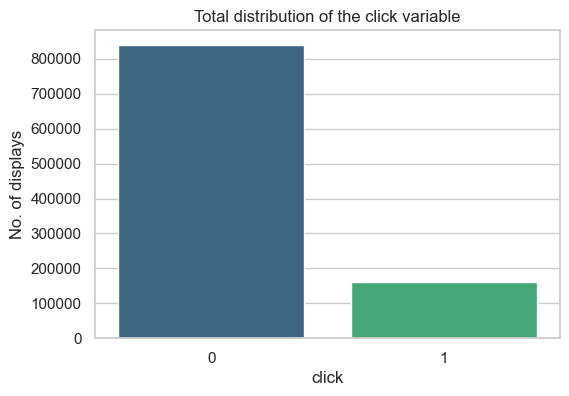
\includegraphics[width=0.9\textwidth]{results/click_distribution.png}
        \captionof{figure}{\small Total distribution of the \texttt{click} variable.}
    \end{column}
\end{columns}
\end{frame}

\begin{frame}{Avazu dataset: EDA vol.2}
\begin{columns}[c]
    \begin{column}{0.4\textwidth}
        \begin{block}{Time dependency}
        \small
        \begin{itemize}
            \item The average CTR is not constant.
            \item Clear fluctuations depend on the hour of the day.
            \item This suggests the presence of natural CD in the stream.
        \end{itemize}
        \end{block}
    \end{column}
    \begin{column}{0.6\textwidth}
        \centering
        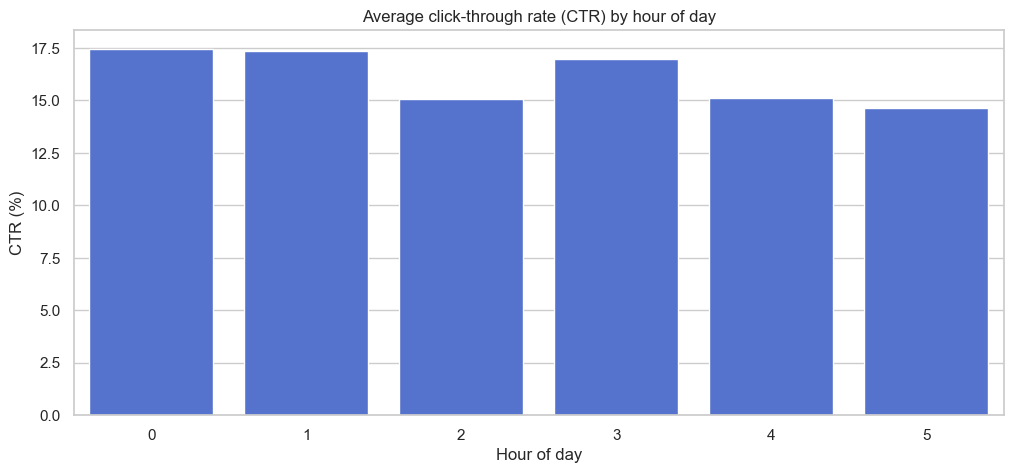
\includegraphics[width=1\textwidth]{results/plot_a.png}
        \captionof{figure}{\small Average CTR by hour of day.}
    \end{column}
\end{columns}
\end{frame}


\begin{frame}{Avazu dataset: EDA vol.3}
\begin{columns}[T]
    \begin{column}{0.5\textwidth}
        \centering
        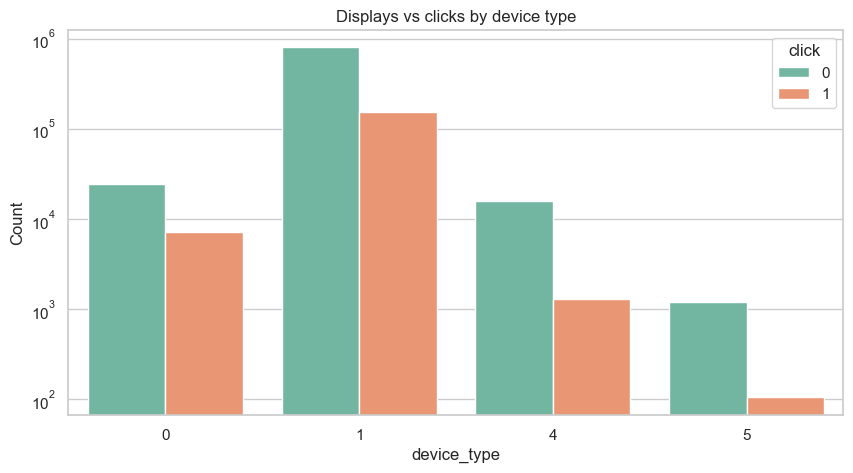
\includegraphics[width=0.95\textwidth]{results/plot_b.png}
        \captionof{figure}{\small Displays vs clicks by device type.}
        \vspace{0.2cm}
        \begin{itemize}
            \item \small \textbf{Device type:} one platform dominates traffic, but propensity to click varies significantly.
        \end{itemize}
    \end{column}
    \begin{column}{0.5\textwidth}
        \centering
        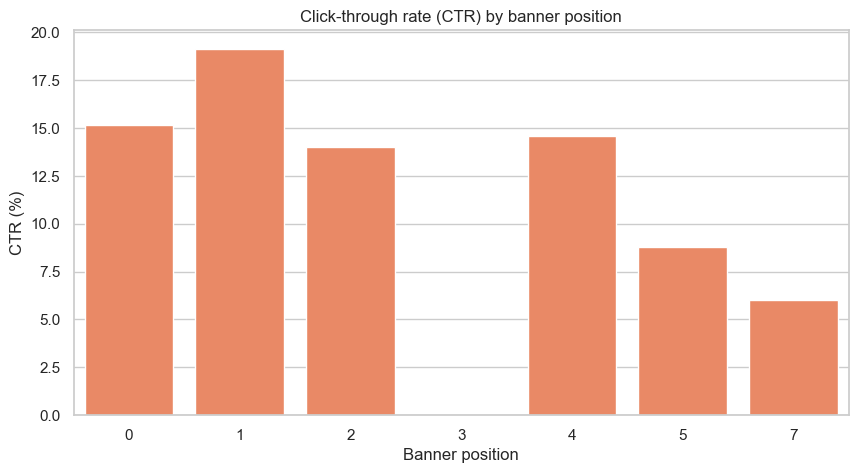
\includegraphics[width=0.95\textwidth]{results/plot_c.png}
        \captionof{figure}{\small CTR by banner position.}
        \vspace{0.2cm}
        \begin{itemize}
            \item \small \textbf{Ad placement:} correlation between physical banner position and CTR.
        \end{itemize}
    \end{column}
\end{columns}
\end{frame}


\begin{frame}{Criteo dataset: EDA vol.1}
\begin{columns}[c]
    \begin{column}{0.5\textwidth}
        \begin{block}{Heterogeneous nature}
        \small
        \begin{itemize}
            \item 40 attributes total. 13 continuous numerical (\texttt{I1-I13}) and 26 anonymized categorical (\texttt{C1 - C26}).
            \item Sample of 1,000,000 instances.
            \item \textbf{Class imbalance:} 25.49\% clicks vs 74.51\% non-clicks.
        \end{itemize}
        \end{block}
    \end{column}
    \begin{column}{0.5\textwidth}
        \centering
        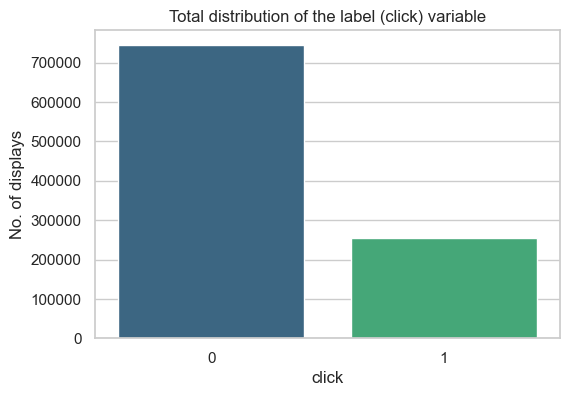
\includegraphics[width=0.9\textwidth]{results/criteo_click_distrbution.png}
        \captionof{figure}{\small Total distribution of the \texttt{label} variable.}
    \end{column}
\end{columns}
\end{frame}

\begin{frame}{Criteo dataset: EDA vol.2}
\begin{columns}[c]
    \begin{column}{0.4\textwidth}
        \begin{alertblock}{Data sparsity}
        \small
        \begin{itemize}
            \item Presence of missing values (NaNs) across numerical columns (\texttt{I12} missing $\sim$75\%).
            \item Requires zero-imputation.
        \end{itemize}
        \end{alertblock}
        \begin{block}{Numerical skewness}
        \small
        \begin{itemize}
            \item Heavily right-skewed, long-tail distributions.
        \end{itemize}
        \end{block}
    \end{column}
    \begin{column}{0.6\textwidth}
        \centering
        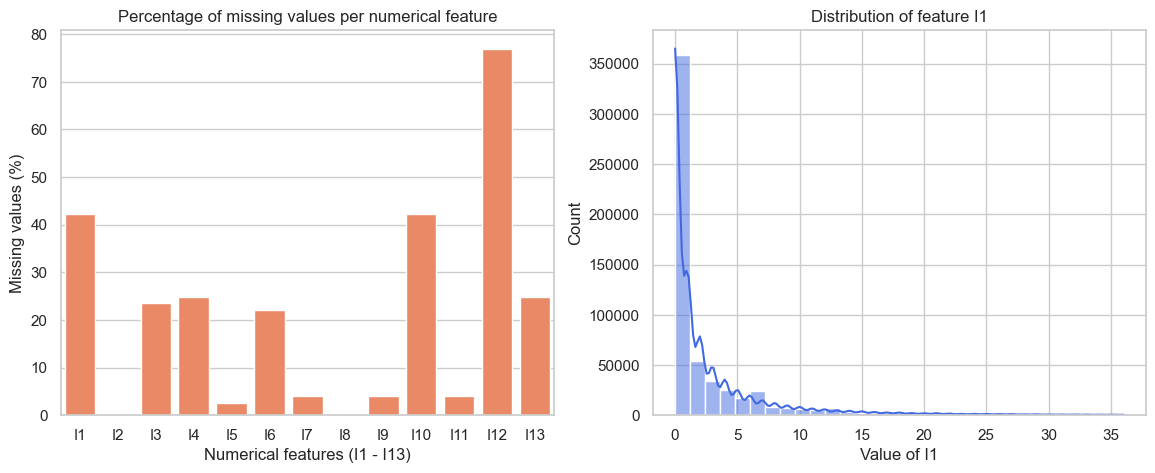
\includegraphics[width=1\textwidth]{results/missing_and_skew.png}
        \captionof{figure}{\small Missing values (left) and feature I1 skewness (right).}
    \end{column}
\end{columns}
\end{frame}


\begin{frame}{Feature engineering and hashing}
    \begin{block}{Temporal and rolling window features}
    \small
    \begin{itemize}
        \item \textbf{Avazu:} extracted specific time details and interaction features (\texttt{site\_x\_hour}). Implemented a sliding window ($W=1000$).
        \item \textbf{Criteo:} Applied sliding window ($W=1000$) to the first five numerical columns to compute moving averages, standard deviations, and deviations from the mean.
    \end{itemize}
    \end{block}

    \begin{block}{Dimensionality reduction via feature hashing \cite{weinberger2009feature}}
    \small
    \begin{itemize}
        \item Used \texttt{FeatureHasher} to compress millions of categorical strings into a fixed-size vector of exactly 100 columns.
        \item Constant memory use, faster training times.
    \end{itemize}
    \end{block}
\end{frame}


\begin{frame}{Synthetic stream: Agrawal generator \cite{agrawal1993database}}
\begin{columns}[T]
    \begin{column}{0.5\textwidth}
        \begin{block}{Why synthetic data?}
        \small Measuring the exact speed of adaptation requires a 100\% controlled environment.
        \end{block}
        \begin{itemize}
            \small
            \item Simulates loan approvals (9 continuous attributes).
            \item Total length: 1,000,000 instances.
        \end{itemize}
    \end{column}
    \begin{column}{0.5\textwidth}
        \begin{alertblock}{Abrupt drift injection (in MOA \cite{bifet2010moa})}
        \small
        \begin{itemize}
            \item \textbf{Instances 1 -- 500,000:}\\ function 1 (stable learning).
            \item \textbf{Instance 500,001:}\\ sudden shift to function 2.
            \item \textbf{Instances 500,000 -- 1M:}\\ old rules become obsolete.
        \end{itemize}
        \end{alertblock}
    \end{column}
\end{columns}
\end{frame}


\begin{frame}{Empirical drift verification (Avazu)}
\begin{columns}[c]
    \begin{column}{0.4\textwidth}
        \begin{block}{ADWIN algorithm \cite{bifet2007learning, bifet2009adaptive}}
        \small
        \begin{itemize}
            \item Verifying that CTR streams are truly non-stationary.
            \item Local CTR fluctuates significantly (14\% to 18.5\%).
            \item 4 distinct CD alerts triggered in 1M instances.
        \end{itemize}
        \end{block}
    \end{column}
    \begin{column}{0.6\textwidth}
        \centering
        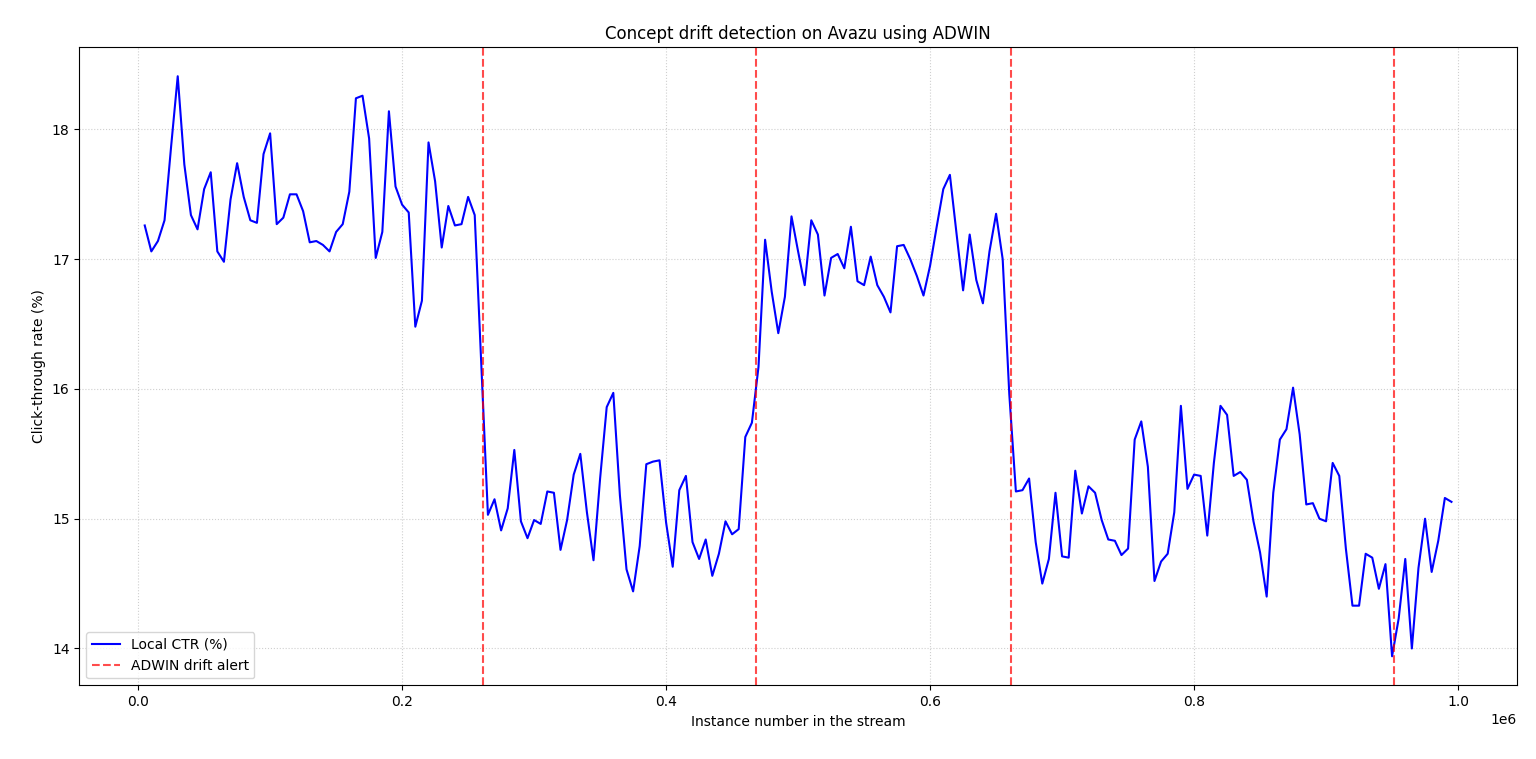
\includegraphics[width=1\textwidth]{results/CD_avazu.png}
        \captionof{figure}{\small Concept drift detection on Avazu.}
    \end{column}
\end{columns}
\end{frame}


\begin{frame}{Empirical drift verification (Criteo)}
\begin{columns}[c]
    \begin{column}{0.4\textwidth}
        \begin{block}{Criteo volatility}
        \small
        \begin{itemize}
            \item CTR rapidly climbs from initial values around 21\% up to nearly 28\%.
            \item 3 major drift alerts triggered.
            \item  Natural drifts are prevalent, exposing the need for dynamic online learning models.
        \end{itemize}
        \end{block}
    \end{column}
    \begin{column}{0.6\textwidth}
        \centering
        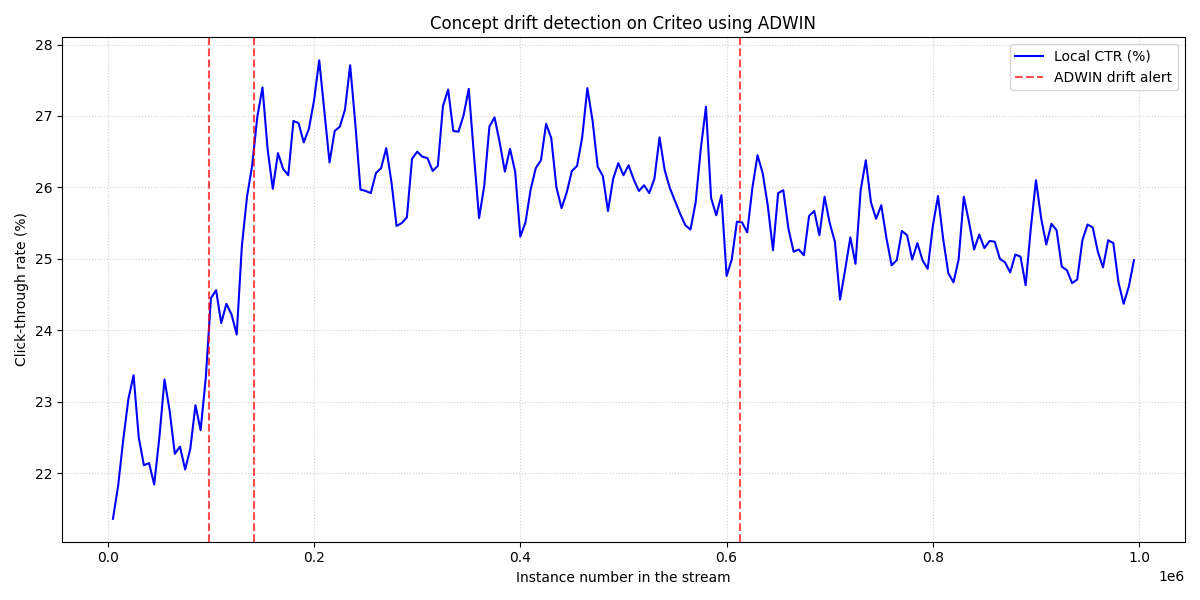
\includegraphics[width=1\textwidth]{results/CD_criteo.png}
        \captionof{figure}{\small Concept drift detection on Criteo.}
    \end{column}
\end{columns}
\end{frame}


\begin{frame}{The adaptation gap}
\begin{columns}[c]
    \begin{column}{0.45\textwidth}
        \begin{itemize}
            \small
            \item \textbf{Baseline:} Hoeffding Adaptive Tree (HAT).
            \item Abrupt drift injected exactly at 500k.
            \item Error spikes abruptly to $>30\%$. 
            \item The subsequent slow recovery forms a distinct triangle of error.
            \item Standard trees are reactive and slow. OFS aims to flatten this curve and minimize $t_{recovery}$.
        \end{itemize}
    \end{column}
    \begin{column}{0.55\textwidth}
        \centering
        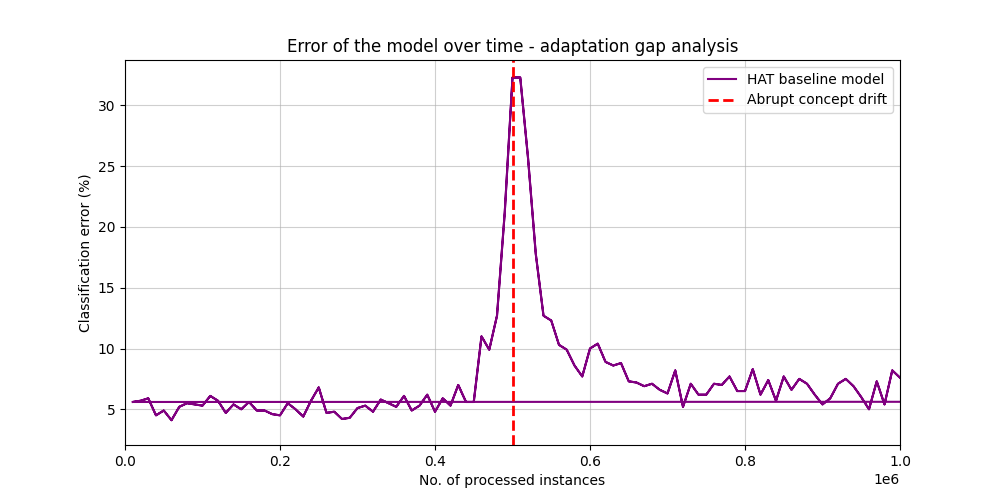
\includegraphics[width=1\textwidth]{results/adaptation_gap.png}
        \captionof{figure}{\small Error spike and recovery time ($t_{recovery}$).}
    \end{column}
\end{columns}
\end{frame}

% -- CZĘŚĆ OGANA
\begin{frame}{Solution architecture: stream pipeline}
\centering
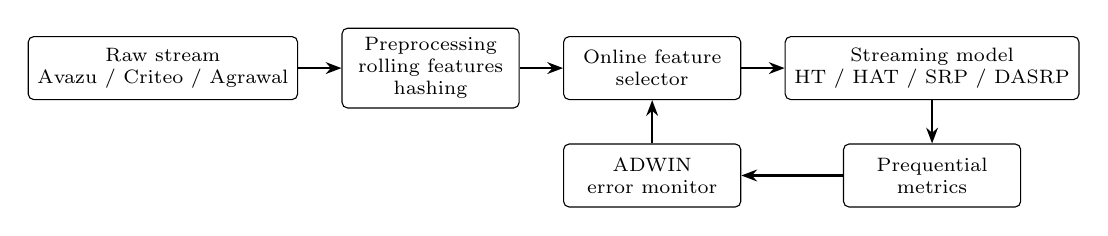
\begin{tikzpicture}[
    node distance=0.55cm and 0.55cm,
    every node/.style={font=\scriptsize},
    box/.style={draw, rounded corners=2pt, align=center, minimum width=2.25cm, minimum height=0.8cm},
    arrow/.style={-{Stealth[length=2mm]}, thick}
]
    \node[box] (data) {Raw stream\\Avazu / Criteo / Agrawal};
    \node[box, right=of data] (features) {Preprocessing\\rolling features\\hashing};
    \node[box, right=of features] (selector) {Online feature\\selector};
    \node[box, right=of selector] (model) {Streaming model\\HT / HAT / SRP / DASRP};
    \node[box, below=of model] (metrics) {Prequential\\metrics};
    \node[box, below=of selector] (adwin) {ADWIN\\error monitor};

    \draw[arrow] (data) -- (features);
    \draw[arrow] (features) -- (selector);
    \draw[arrow] (selector) -- (model);
    \draw[arrow] (model) -- (metrics);
    \draw[arrow] (metrics) -- (adwin);
    \draw[arrow] (adwin) -- (selector);
\end{tikzpicture}

\vspace{0.25cm}
\begin{columns}[T]
    \begin{column}{0.48\textwidth}
        \begin{block}{Common path}
        \small
        Each instance is transformed once, filtered to the currently active feature subset, predicted, scored, and then used for training.
        \end{block}
    \end{column}
    \begin{column}{0.48\textwidth}
        \begin{block}{Feedback loop}
        \small
        ADWIN observes the online error stream. A drift alarm triggers feature re-ranking instead of waiting for a fixed retraining batch.
        \end{block}
    \end{column}
\end{columns}
\end{frame}

\begin{frame}{Solution architecture: drift-aware SRP}
\begin{columns}[T]
    \begin{column}{0.5\textwidth}
        \begin{block}{Adaptation logic}
        \small
        \begin{enumerate}
            \item Keep a pre-drift window of recent instances.
            \item After ADWIN fires, collect a post-drift window.
            \item Recompute Information Gain for both windows.
            \item Treat falling-IG features as weak and rising-IG features as strong.
            \item Replace weak features inside affected ensemble subspaces.
        \end{enumerate}
        \end{block}
    \end{column}
    \begin{column}{0.5\textwidth}
        \begin{block}{Implementation details}
        \small
        \begin{itemize}
            \item Ensemble: 10 Hoeffding-tree learners.
            \item Real CTR: \texttt{topK}=20, window=5,000, subspace size=20.
            \item Agrawal: \texttt{topK}=5, window=800, subspace size=4.
            \item Only learners whose subspace contains weak features are rebuilt; untouched learners keep their state.
            \item Rebuilt high-overlap learners start at weight 0.3 and recover by 0.001 per instance.
        \end{itemize}
        \end{block}
    \end{column}
\end{columns}
\end{frame}

% -- DODATKOWE SLAJDY: ARCHITEKTURA I METODOLOGIA

\begin{frame}{Prequential evaluation loop}
\begin{columns}[T]
    \begin{column}{0.52\textwidth}
        \begin{block}{Test-then-train protocol}
        \small
        For every stream instance, the model first predicts the label, then the prediction is scored, and only after that the same instance is used for training.
        \end{block}

        \vspace{0.15cm}
        \begin{block}{Why it matters}
        \small
        This avoids leakage from future observations and gives a time-resolved estimate of model quality under changing stream conditions.
        \end{block}
    \end{column}

    \begin{column}{0.48\textwidth}
        \small
        \begin{enumerate}
            \item Read next chronological instance.
            \item Apply feature transformation and selection.
            \item Predict click probability.
            \item Update accuracy, log-loss and AUC.
            \item Send error signal to ADWIN.
            \item Train model on the same instance.
        \end{enumerate}
    \end{column}
\end{columns}
\end{frame}


\begin{frame}{Implemented components}
\begin{columns}[T]
    \begin{column}{0.5\textwidth}
        \begin{block}{Data and models}
        \small
        \begin{itemize}
            \item \textbf{Streams}: Avazu, Criteo, Agrawal.
            \item \textbf{Providers}: unified stream interface.
            \item \textbf{Models}: HT, HAT, SRP, DASRP.
            \item \textbf{Evaluation}: common prequential runner.
        \end{itemize}
        \end{block}
    \end{column}

    \begin{column}{0.5\textwidth}
        \begin{block}{Selection and adaptation}
        \small
        \begin{itemize}
            \item No feature selection.
            \item Static top-K after warm-up.
            \item Periodic online Information Gain ranking.
            \item Drift-aware reselection triggered by ADWIN.
            \item Selective subspace repair in DASRP.
        \end{itemize}
        \end{block}
    \end{column}
\end{columns}

\vspace{0.2cm}
\begin{block}{Design goal}
\small
All providers, selectors and models expose common interfaces, so every configuration can be evaluated in the same loop without changing the evaluator.
\end{block}
\end{frame}


\begin{frame}{Drift-aware feature selection}
\begin{columns}[T]
    \begin{column}{0.48\textwidth}
        \begin{block}{Before/after comparison}
        \small
        Instead of updating features on a fixed schedule, the selector waits for an ADWIN alarm and compares feature relevance before and after the detected drift.
        \end{block}

        \[
        \Delta IG_i = IG_{after,i} - IG_{before,i}
        \]
    \end{column}

    \begin{column}{0.52\textwidth}
        \begin{block}{Decision rule}
        \small
        \begin{itemize}
            \item Positive $\Delta IG$ means that a feature became stronger.
            \item Negative $\Delta IG$ means that a feature lost relevance.
            \item Strengthened features are added to the active set.
            \item Weakened features are removed from the active set.
            \item The final subset is corrected back to size $K$.
        \end{itemize}
        \end{block}
    \end{column}
\end{columns}

\vspace{0.15cm}
\begin{block}{Main intuition}
\small
The selector reacts to changes in feature usefulness caused by drift, not only to absolute feature rankings at one point in time.
\end{block}
\end{frame}


\begin{frame}{Model reaction to feature reselection}
\begin{columns}[T]
    \begin{column}{0.48\textwidth}
        \begin{block}{HT / HAT path}
        \small
        \begin{itemize}
            \item Feature change creates a new input header.
            \item The whole model is reset.
            \item Previous tree structure is discarded.
            \item Learning starts again from an empty model.
        \end{itemize}
        \end{block}
    \end{column}

    \begin{column}{0.52\textwidth}
        \begin{block}{DASRP path}
        \small
        \begin{itemize}
            \item Each ensemble member owns its own subspace.
            \item Only subspaces containing weak features are changed.
            \item Only heavily affected learners are rebuilt.
            \item Reset learners vote with reduced weight.
            \item Their weight gradually returns to 1.0.
        \end{itemize}
        \end{block}
    \end{column}
\end{columns}

\vspace{0.2cm}
\begin{block}{Key difference}
\small
Monolithic models lose all accumulated knowledge after reselection, while DASRP preserves unaffected learners and adapts only the damaged parts of the ensemble.
\end{block}
\end{frame}

% --- CZĘŚĆ HUBIEGO 
\begin{frame}{Evaluation procedure}
    \begin{block}{Prequential evaluation (test-then-train)}
    \small
    \begin{itemize}
        \item Cross-validation is inapplicable to endless streams.
        \item Each incoming instance is first used to test the model, and only then passed to train the model. 
        \item Provides evaluation on unseen data.
    \end{itemize}
    \end{block}

    \begin{block}{Chosen metrics}
    \small
    \begin{itemize}
        \item \textbf{Logarithmic loss (Log Loss) \cite{vovk2015fundamental}:} heavily penalizes confident yet incorrect predictions.
        \item \textbf{AUC ROC \cite{fawcett2006introduction}:} ability to correctly rank positive vs negative classes.
    \end{itemize}
    \end{block}

    \begin{alertblock}{Experiment scale in this repository}
    \small
    48 experiments: 36 baseline combinations plus 12 drift-aware variants. Each dataset was evaluated for 200,000 instances, with metric snapshots every 1,000 instances.
    \end{alertblock}
\end{frame}

\begin{frame}{Final evaluation: real CTR streams}
\scriptsize
\centering
\begin{tabular}{llccc}
\toprule
Dataset & Method & Accuracy & Log Loss & AUC \\
\midrule
Avazu & SRP + static top-K & 0.8243 & 0.4659 & 0.7022 \\
Avazu & \textbf{DASRP + drift-aware SRP} & \textbf{0.8253} & \textbf{0.4332} & \textbf{0.7048} \\
\midrule
Criteo & SRP + online ranking & 0.7557 & 0.5522 & 0.6512 \\
Criteo & \textbf{DASRP + drift-aware SRP} & \textbf{0.7583} & \textbf{0.5291} & 0.6511 \\
Criteo & SRP + static top-K & \textbf{0.7634} & 0.5622 & \textbf{0.6754} \\
\bottomrule
\end{tabular}

\vspace{0.35cm}
\begin{columns}[T]
    \begin{column}{0.48\textwidth}
        \begin{block}{Main gain}
        \small
        DASRP achieved the lowest Log Loss on both real CTR streams: 7.0\% lower than the best Avazu baseline and 4.2\% lower than the best Criteo Log Loss baseline.
        \end{block}
    \end{column}
    \begin{column}{0.48\textwidth}
        \begin{alertblock}{Important nuance}
        \small
        On Criteo, static SRP still produced the best AUC and accuracy. The proposed method mainly improved probability calibration.
        \end{alertblock}
    \end{column}
\end{columns}
\end{frame}

\begin{frame}{Real CTR: final Log Loss visualized}
\begin{columns}[c]
    \begin{column}{0.66\textwidth}
        \centering
        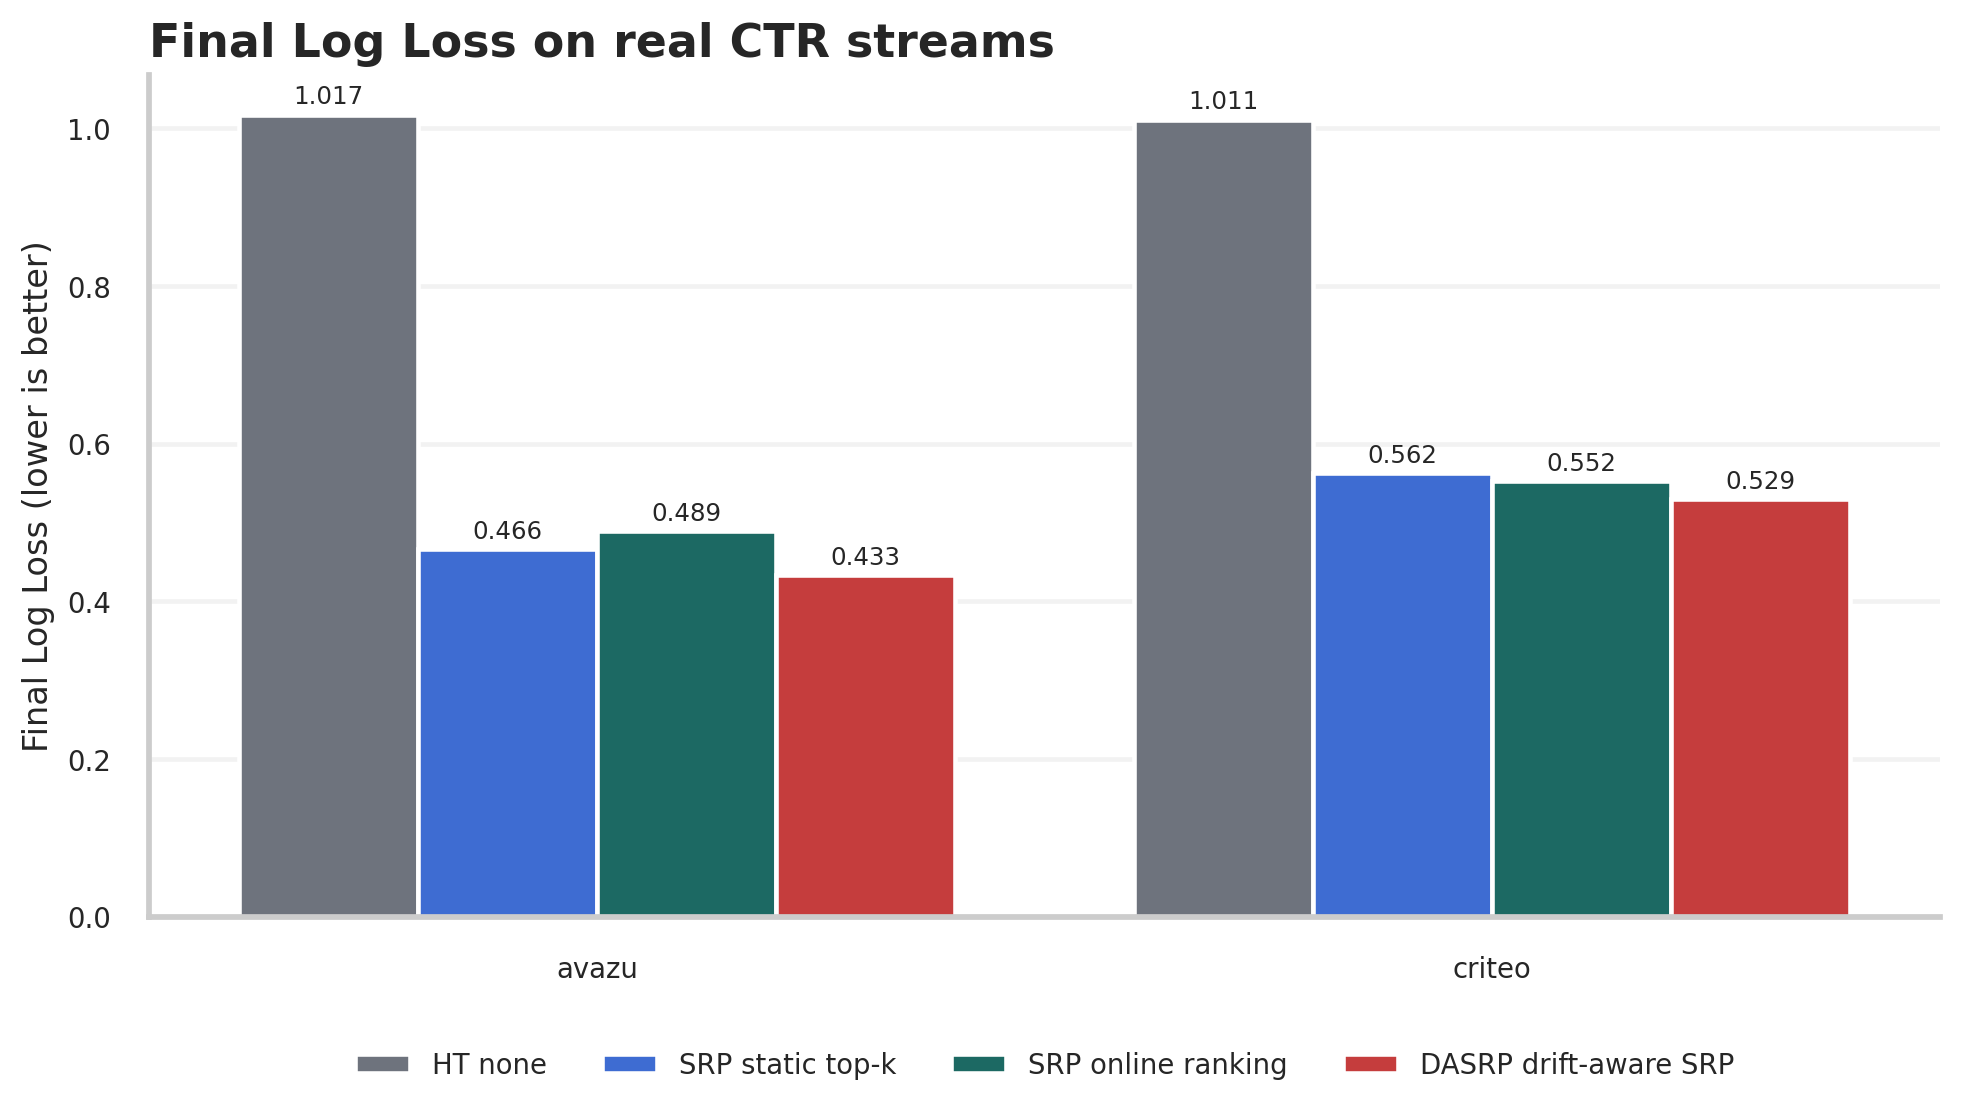
\includegraphics[width=\textwidth,height=0.62\textheight,keepaspectratio]{results/evaluation/eval_real_final_logloss.png}
    \end{column}
    \begin{column}{0.34\textwidth}
        \begin{block}{Main message}
        \scriptsize
        \begin{itemize}
            \item DASRP obtains the lowest final Log Loss on both real CTR datasets.
            \item Avazu: 0.433 vs 0.466 for the best SRP baseline.
            \item Criteo: 0.529 vs 0.552 for the best Log Loss baseline.
        \end{itemize}
        \end{block}
        \begin{alertblock}{Interpretation}
        \scriptsize
        The strongest improvement is probability calibration, not only class accuracy.
        \end{alertblock}
    \end{column}
\end{columns}
\end{frame}

\begin{frame}{Evaluation dynamics: real CTR streams}
\centering
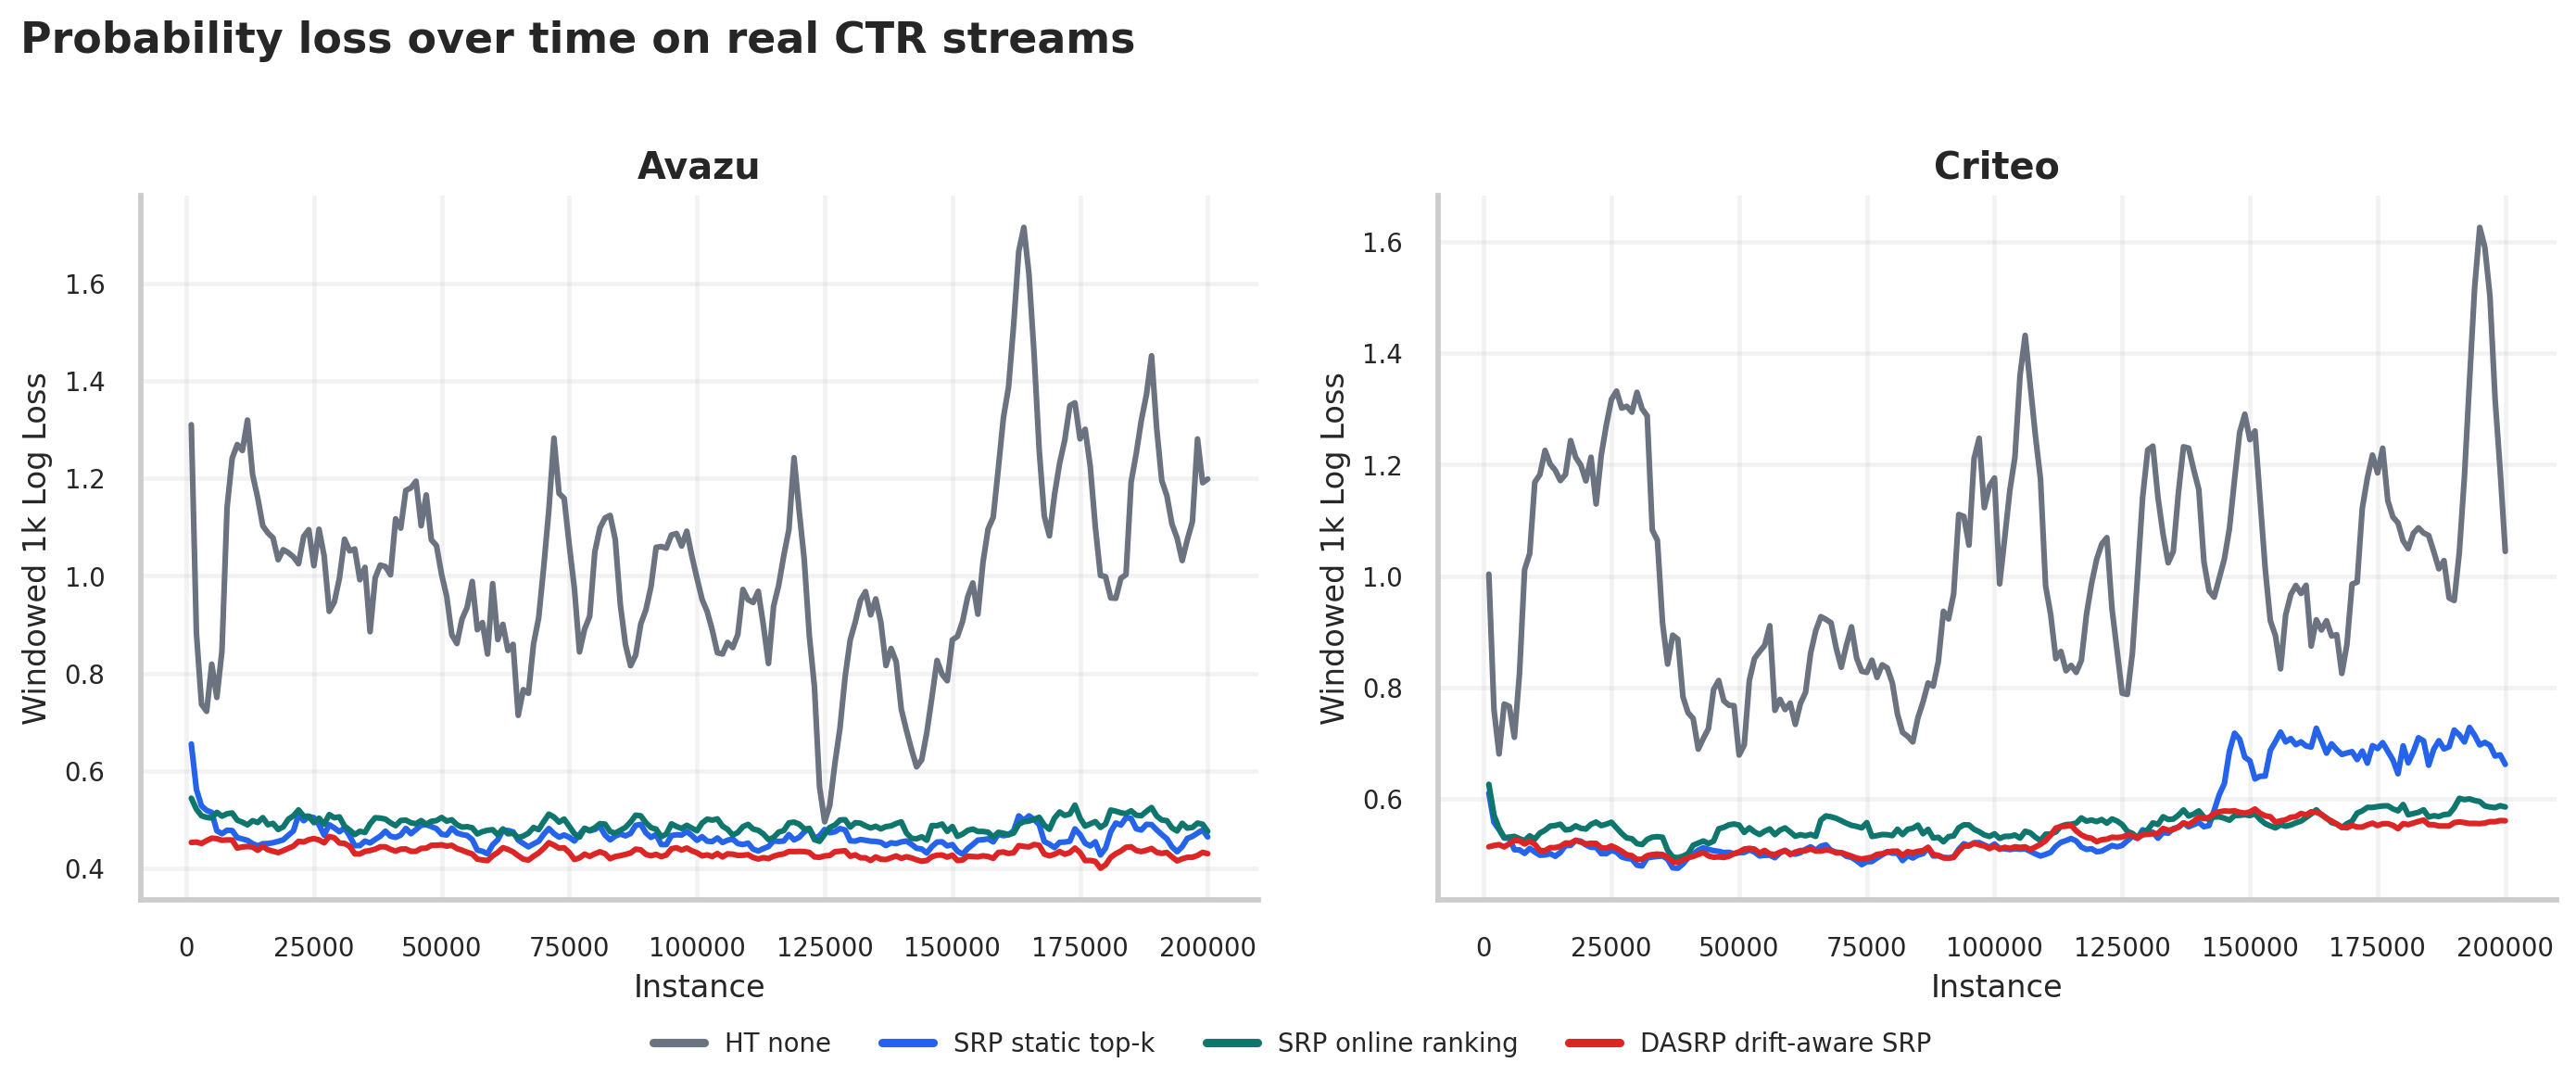
\includegraphics[width=0.95\textwidth,height=0.66\textheight,keepaspectratio]{results/evaluation/eval_real_windowed_logloss.png}

\vspace{-0.05cm}
\begin{block}{What the curves show}
\scriptsize
DASRP stays among the lowest-loss methods throughout the stream. The gain is especially visible on Avazu, while Criteo shows a later degradation of static SRP that DASRP avoids.
\end{block}
\end{frame}

\begin{frame}{Runtime comparison}
\begin{columns}[c]
    \begin{column}{0.67\textwidth}
        \centering
        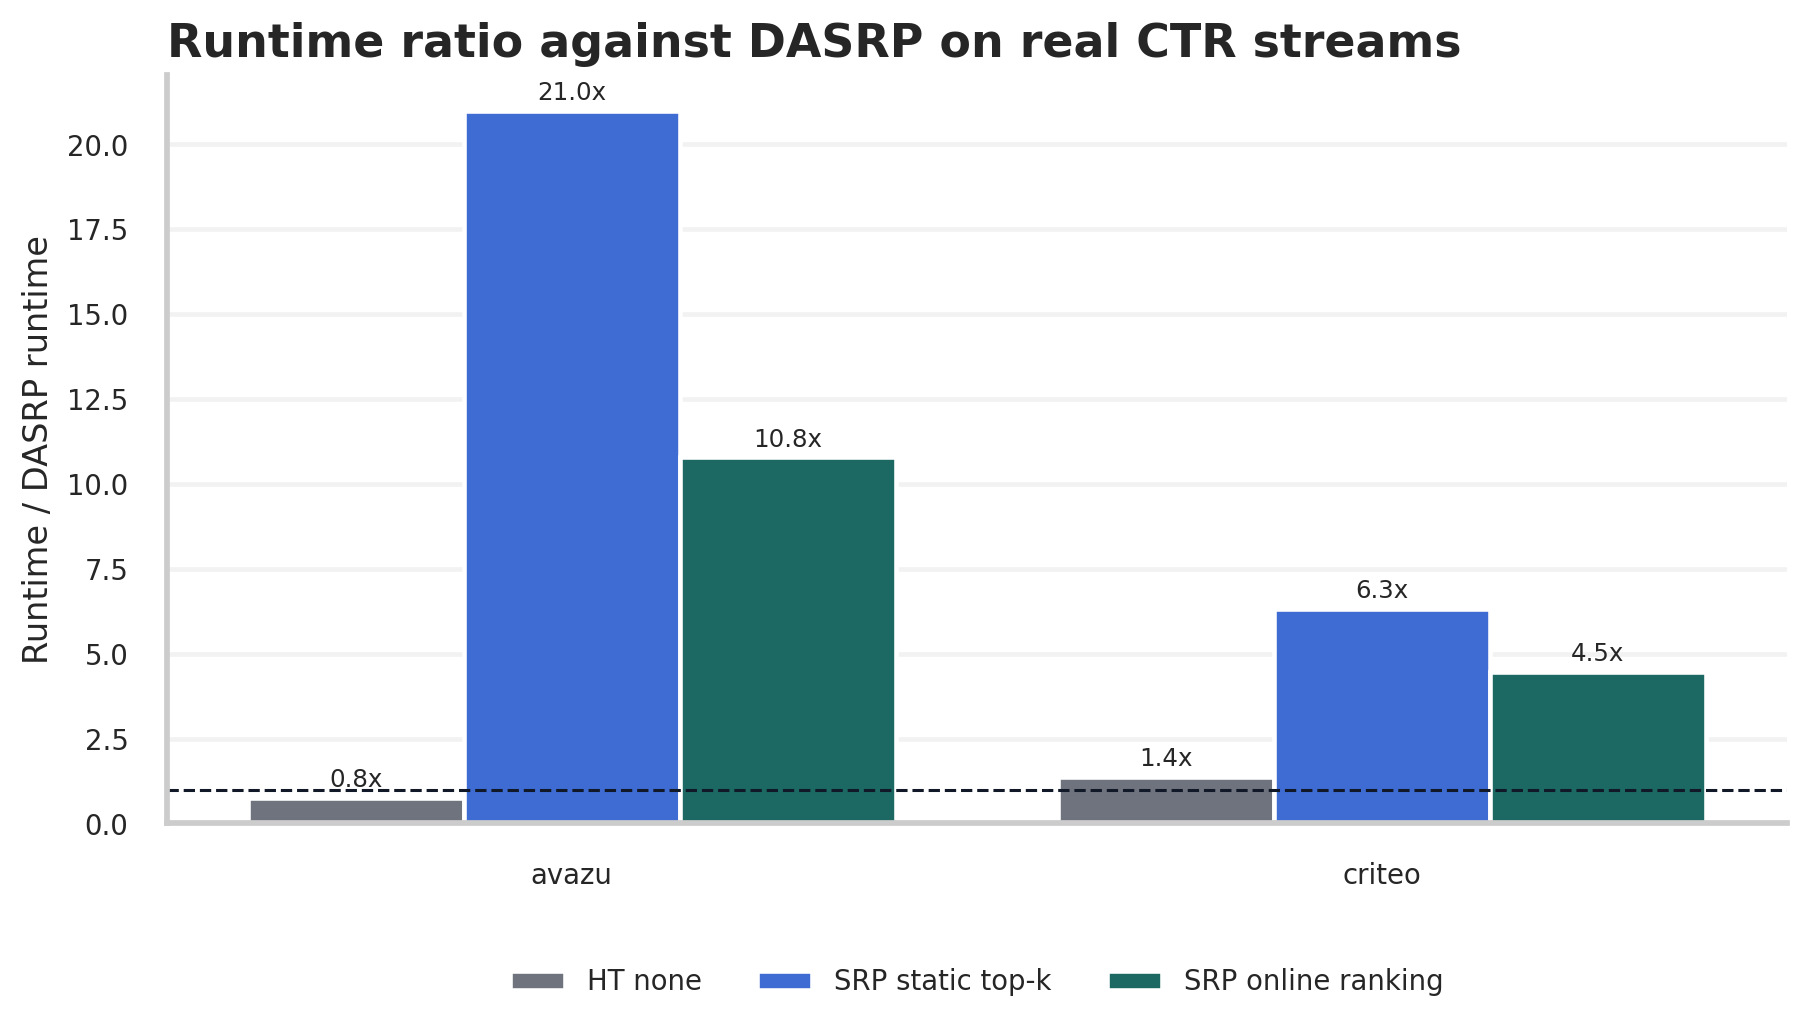
\includegraphics[width=\textwidth,height=0.62\textheight,keepaspectratio]{results/evaluation/eval_real_speedup_vs_dasrp.png}
    \end{column}
    \begin{column}{0.33\textwidth}
        \begin{block}{Why it matters}
        \scriptsize
        \begin{itemize}
            \item Real CTR experiments are high-dimensional after hashing and rolling features.
            \item On Avazu, SRP static top-K took about 21x the DASRP runtime.
            \item HT is faster but less competitive in final Log Loss.
        \end{itemize}
        \end{block}
    \end{column}
\end{columns}
\end{frame}

\begin{frame}{Final evaluation: synthetic drift}
\scriptsize
\centering
\begin{tabular}{llccc}
\toprule
Dataset & Method & Accuracy & Log Loss & AUC \\
\midrule
Sudden Agrawal & HAT + no selector & \textbf{0.9559} & \textbf{0.1604} & 0.9966 \\
Sudden Agrawal & HT + online ranking & 0.9279 & 0.1939 & \textbf{0.9982} \\
Sudden Agrawal & DASRP + drift-aware SRP & 0.8435 & 0.4553 & 0.8838 \\
\midrule
Gradual Agrawal & HT + online ranking & 0.9195 & \textbf{0.2171} & 0.9979 \\
Gradual Agrawal & HAT + no selector & \textbf{0.9282} & 0.2420 & 0.9975 \\
Gradual Agrawal & DASRP + drift-aware SRP & 0.8029 & 0.4848 & 0.9067 \\
\bottomrule
\end{tabular}

\vspace{0.35cm}
\begin{block}{Interpretation}
\small
In the low-dimensional Agrawal setting, standard adaptive trees and periodic online ranking already recover very well. Drift-aware selection generated many extra alarms, so the proposed mechanism needs stricter tuning for simple synthetic streams.
\end{block}
\end{frame}

\begin{frame}{Synthetic drift: adaptation curves}
\centering
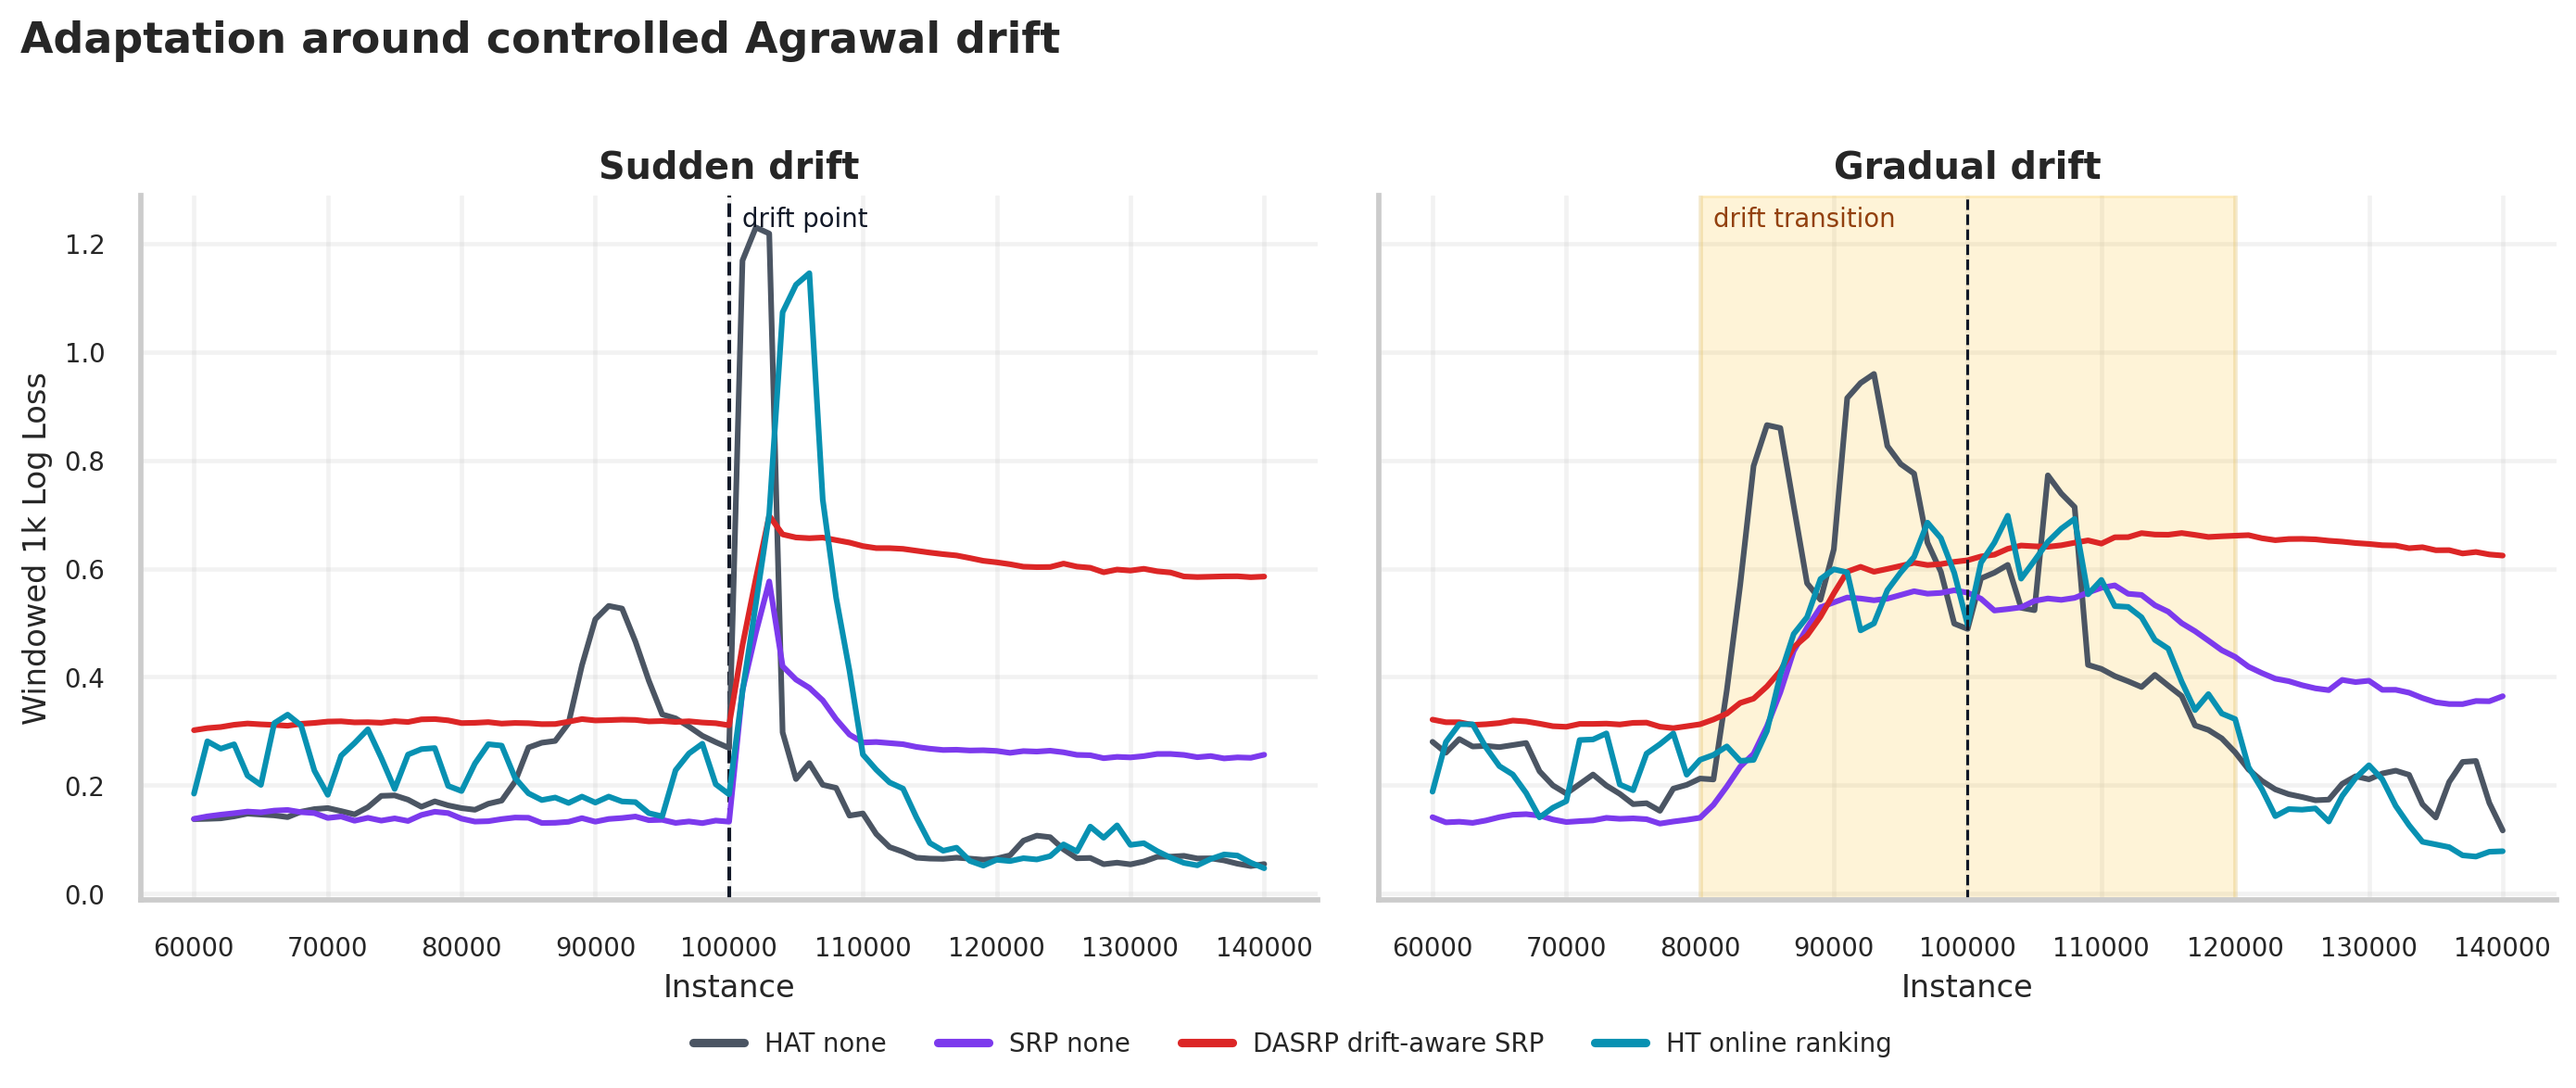
\includegraphics[width=0.95\textwidth,height=0.62\textheight,keepaspectratio]{results/evaluation/eval_synthetic_adaptation.png}

\vspace{-0.05cm}
\begin{block}{Interpretation}
\scriptsize
Standard adaptive trees and periodic online ranking recover quickly on low-dimensional Agrawal streams. DASRP is more conservative here, so its drift thresholds need separate tuning for simple synthetic data.
\end{block}
\end{frame}


\begin{frame}{Conclusion}
\begin{columns}[T]
    \begin{column}{0.5\textwidth}
        \begin{block}{What worked}
        \small
        \begin{itemize}
            \item Feature hashing and rolling features gave a fixed-memory CTR stream representation.
            \item Drift-triggered feature adaptation improved real-stream Log Loss.
            \item DASRP kept unaffected learners alive instead of resetting the whole ensemble.
        \end{itemize}
        \end{block}
    \end{column}
    \begin{column}{0.5\textwidth}
        \begin{alertblock}{What remains}
        \small
        \begin{itemize}
            \item Tune ADWIN delta, window size, and IG threshold per data regime.
            \item Quantify recovery time and area under the loss spike around drift events.
            \item Test larger ensembles and full 1M-instance CTR runs.
        \end{itemize}
        \end{alertblock}
    \end{column}
\end{columns}

\vspace{0.25cm}
\begin{block}{Takeaway}
\small
Online feature selection is most useful when the stream is high-dimensional and feature relevance drifts. In this project, the strongest evidence is on Avazu and Criteo, where DASRP delivers the best probability-aware loss.
\end{block}
\end{frame}


\begin{frame}[allowframebreaks]{References}
    \bibliographystyle{unsrt}
    \bibliography{reference}
\end{frame}

\begin{frame}
    \Huge{\centerline{\textbf{Thank You for Your Attention!}}}
    \vspace{1cm}
    \large{\centerline{Feel free to ask questions :) }}
\end{frame}


\end{document}
